\section{Results}
\label{sec:results}

\subsection{Gold evidence improves aggregate accuracy}
\label{sec:rq1}
Table~\ref{tab:accuracy} answers RQ1.
On the same 10{,}000 claims, designated gold evidence raises GPT-5.4 accuracy from 88.69\% to 96.04\% ($+7.35$~pp) and GPT-5.4-mini from 84.67\% to 95.54\% ($+10.87$~pp).
Paired McNemar tests are large (GPT-5.4 $\chi^2=558.3$, $p\approx 2\times 10^{-123}$; mini $\chi^2=849.1$, $p\approx 10^{-186}$).
Figure~\ref{fig:transitions} shows the four-way transition structure behind those averages.
Evidence also increases cross-model prediction agreement, from 89.3\% ($\kappa=0.786$) without evidence to 97.2\% ($\kappa=0.944$) with evidence.

\begin{figure}[t]
\centering
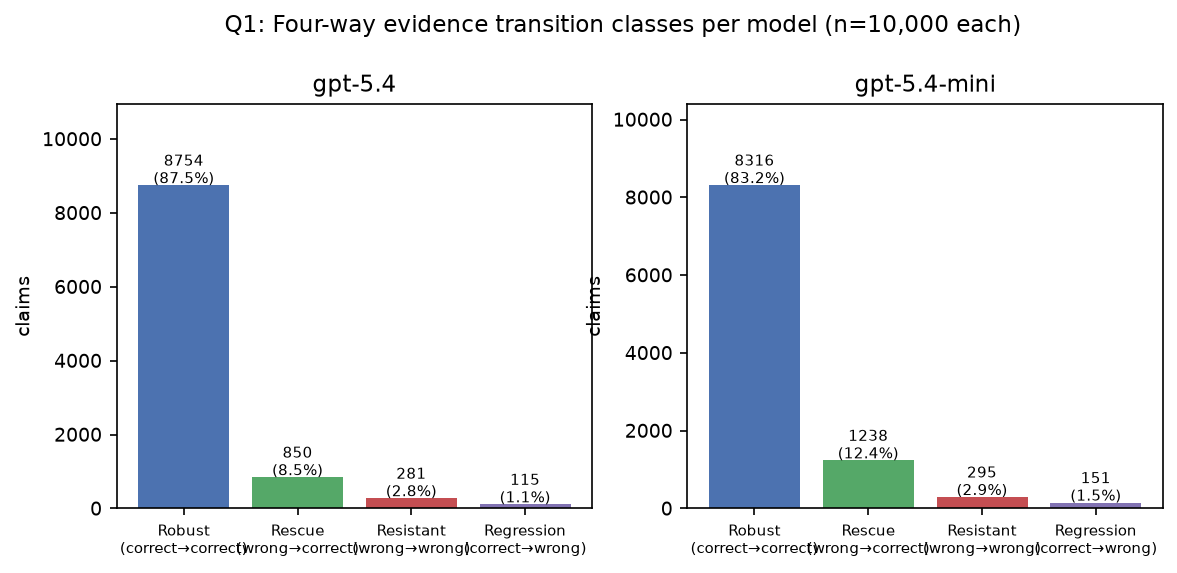
\includegraphics[width=0.92\linewidth]{../analysis_v2/figures/fig1_transition_matrices.png}
\caption{Paired transition matrices for GPT-5.4 and GPT-5.4-mini. Off-diagonal cells are rescues (wrong$\rightarrow$correct) and regressions (correct$\rightarrow$wrong).}
\label{fig:transitions}
\end{figure}

\subsection{Evidence can induce correct-to-wrong regressions}
\label{sec:rq2}
The same paired design produces 115 GPT-5.4 regressions (1.15\%, bootstrap 95\% CI $[0.95,1.36]$) and 151 mini regressions (1.51\%, CI $[1.28,1.75]$).
Rescues are more common: 850 (8.5\%) and 1{,}238 (12.4\%).
Among claim-only errors, evidence corrects 75.2\% (GPT-5.4) and 80.8\% (mini).

Unique-claim counts, not model-observations, are the regression cohort for later adjudication: 226 claims regress for at least one model, 40 for both, and 186 for exactly one (75 GPT-5.4-only, 111 mini-only).
A paired McNemar test on discordant claims finds a modest model difference in regression incidence (115 vs.\ 151, $\chi^2=6.59$, $p=0.010$).
87.3\% of claims share the same transition class across models.
RQ2's answer is therefore: regressions are real, rare relative to 10{,}000 claims, only partly shared, and large enough to study as a structured minority.

\subsection{Characteristics of evidence-induced regressions}
\label{sec:rq3-nli}
Regressions are not a random slice of the sample.
A local NLI diagnostic (nli-deberta-v3-small) disagrees with the FEVER label on 74.8\% of GPT-5.4 regressions and 76.8\% of mini regressions, against 22.6\% of GPT-5.4 robust successes (Figure~\ref{fig:nli}).
Resistant failures look similar (75.8\%).
A second, architecturally different NLI model reproduces the same ordering.
The 2{,}462 claims flagged as weakly warranted also have lower claim-only GPT-5.4 accuracy (81.0\% vs.\ 88.69\%), so the NLI signal marks hard items rather than a quirk of one evidence-condition model.

\begin{figure}[t]
\centering
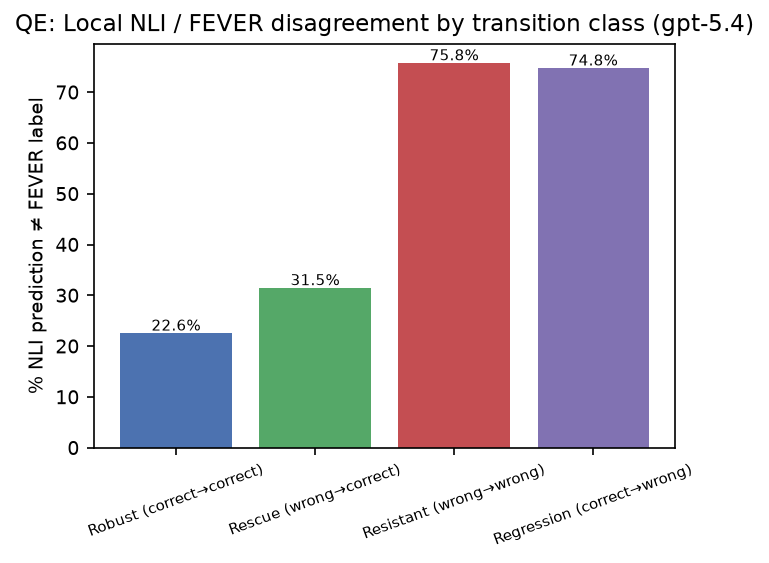
\includegraphics[width=0.88\linewidth]{../analysis_v2/figures/fig6_nli_disagreement.png}
\caption{Local NLI disagreement with the FEVER label by GPT-5.4 transition class. The NLI models are diagnostics, not a relabeling of FEVER.}
\label{fig:nli}
\end{figure}

Label asymmetry is model-dependent.
GPT-5.4 regressions concentrate on Supported claims (88 vs.\ 27 Refuted, $p=1.8\times 10^{-8}$); mini shows no such split (74 vs.\ 77, $p=0.87$).
Surface features (length, overlap, evidence-set size) only weakly separate regressions.
Predictive models that include NLI features do better than surface-only models, but rare-class PR-AUC remains low.
We treat this block as characterization, not as the failure-mode decomposition.

\subsection{Progressive disclosure reveals a mixed failure picture}
\label{sec:rq3-grok}
The Cursor/Grok panel judges the 1{,}061-claim cohort (judged $N=1{,}060$).
Among the 226 regressions, the rule-based taxonomy yields a mixed assignment (Table~\ref{tab:mechanism-grok}): 50.0\% evidence-utilization failure, 11.9\% representation-sensitive, 38.1\% residual ambiguity.
Utilization failure means the panel reaches a high-consensus decisive Stage~C verdict on evidence the GPT model used incorrectly.
Residual ambiguity means the panel remains Ambiguous or Unresolved after structured evidence.
Representation-sensitive items become decisive only after titles or structure are added.

Progressive disclosure itself resolves only a minority of regression ambiguity (7.1\% by titles, 5.3\% only by structure).
No decisive consensus is reversed by later disclosure.
Shared GPT regressions remain more often non-decisive than model-specific ones (Table~\ref{tab:shared}).
This is the Grok answer to RQ3: a mixture, with utilization largest and representation smallest, not a single-cause story.

\subsection{Supporting cross-family checks}
\label{sec:supporting}
GLM-5.3 Stage~A, compared with frozen Cursor Stage~A on 1{,}060 items, yields modal verdict agreement 0.862 and consensus agreement 0.831.
GLM is less ambiguity-conservative (ambiguous/unresolved rate 0.223 vs.\ Cursor 0.291).
This is Stage~A robustness only.

The Claude residual Stage~C test on 231 Grok leftovers finds persistent ambiguity on 134/231 (58.0\%, CI $51.5$--$64.1$) and Claude-resolved Grok leftovers on 97/231 (42.0\%).
The leftover set is therefore mixed: most of it still looks underdetermined to a second family, and a large high-consensus slice does not.
This experiment cannot re-open the 113 Grok utilization failures or the 27 representation-sensitive items, because those items were not in the residual sample.

\subsection{Full Claude replication}
\label{sec:rq4}
The complete Claude A$\rightarrow$B$\rightarrow$C panel judges all 226 regressions from scratch (3{,}390 judgments).
Table~\ref{tab:cross-family} and Figure~\ref{fig:by-family} are the study-level comparison.
Claude assigns 65.9\% utilization failure (149), 5.3\% representation-sensitive (12), and 28.8\% residual ambiguity (65).
The rank order matches Grok.
The magnitudes do not: Claude's utilization share is 15.9~pp higher, and the reported 95\% intervals (Claude $59.5$--$71.8$; Grok $43.5$--$56.5$) do not overlap.

\begin{figure}[t]
\centering
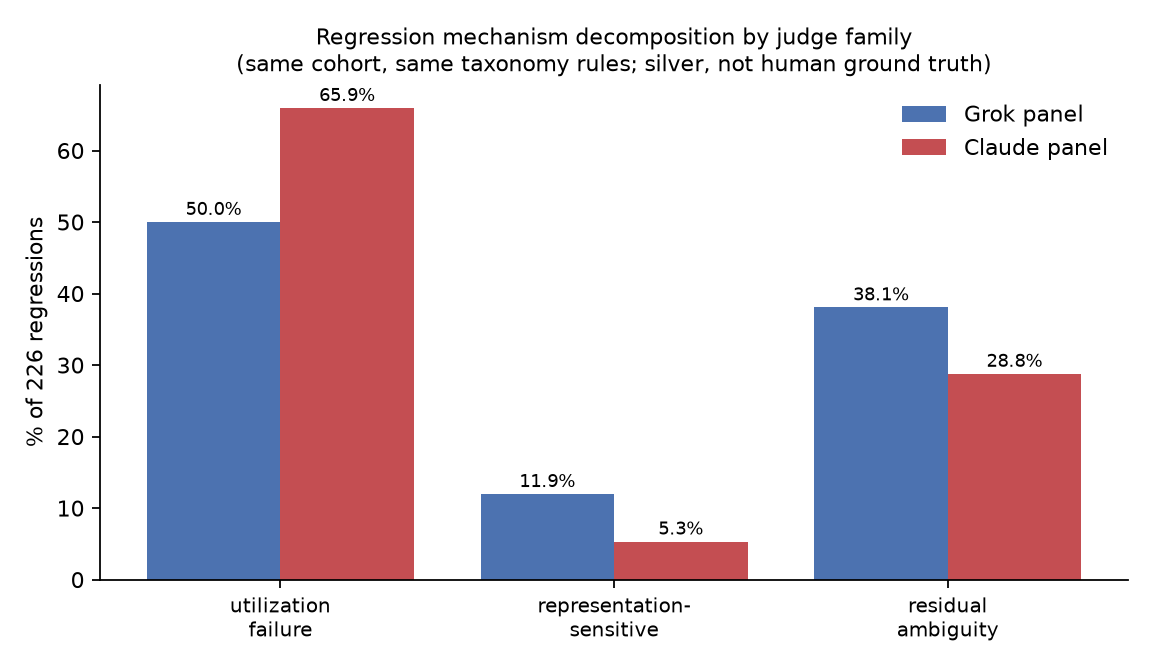
\includegraphics[width=0.92\linewidth]{../silver_adjudication_v1/claude_full_regression_panel/figures/fig1_mechanism_by_family.png}
\caption{Diagnostic category shares for the same 226 regressions under Cursor/Grok and Claude. Ordering matches; prevalences do not.}
\label{fig:by-family}
\end{figure}

Exact taxonomy agreement is 74.3\% (168/226); broad-category agreement is also 74.3\%, because neither panel assigns \texttt{silver\_title\_context\_sensitive}.
Cohen's $\kappa=0.537$ (moderate).
Disagreement is directional.
Claude reclassifies 20 of Grok's 27 representation-sensitive items and 22 of Grok's 86 residual items as utilization failures, and moves only six items the other way.
Claude retains 4 of Grok's 27 representation-sensitive cases.

\begin{figure}[t]
\centering
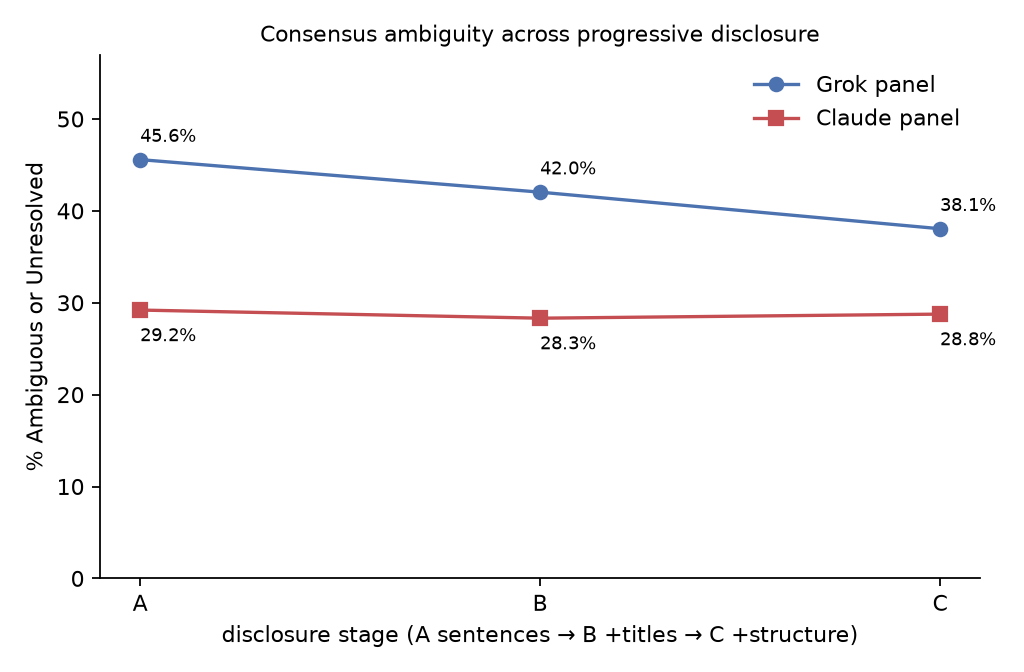
\includegraphics[width=0.88\linewidth]{../silver_adjudication_v1/claude_full_regression_panel/figures/fig2_stage_ambiguity.png}
\caption{Stage-wise non-decisive rates on the 226 regressions. Claude is more decisive at every stage; the gap narrows from Stage~A to Stage~C. Title and structure disclosure resolve only a small share in both families.}
\label{fig:stage-amb}
\end{figure}

Figure~\ref{fig:stage-amb} shows the stage-level mechanism behind that shift.
Claude's ambiguity rate is lower at every stage (29.2\% / 28.3\% / 28.8\% vs.\ Grok 45.6\% / 42.0\% / 38.1\%; McNemar $p=7.8\times 10^{-10}$, $3.4\times 10^{-7}$, $7.5\times 10^{-4}$).
Title and structure resolution rates do not differ significantly across families.
Neither family reverses a decisive consensus after added disclosure.
Shared regressions remain stickier than model-specific ones under Claude as well (Table~\ref{tab:shared}).

\subsection{What replicates and what does not}
\label{sec:what-replicates}
Robust across both complete panels: all three diagnostic categories occur; utilization failure is largest; residual ambiguity remains substantial; representation-sensitive cases are smallest; additional disclosure resolves only a minority; decisive consensus is never reversed; shared regressions are more ambiguity-prone.

Quantitatively offset but directionally consistent: the utilization-versus-residual split, and stage-wise ambiguity (same trend, 9--16~pp lower under Claude).

Judge-family-sensitive: absolute ambiguity at every stage; the representation-sensitive item set (4-item overlap); and per-claim assignment ($\kappa=0.537$).
RQ4's answer is therefore qualitative yes, quantitative no.
The design cannot decide whether Claude is better calibrated or more overconfident on thin warrants, because both panels are models scoring the same packets.
